\section{Introduction}

The COVID-19 pandemic, as a global public health crisis, has precipitated unprecedented societal, economic, and political disruptions, underscoring the imperative of real-time epidemic forecasting. However, many of the epidemic surveillance values published by public health surveillance data systems are often and repeatedly revised in subsequent releases after their first release, and do not accurately reflect disease activity in real time. This often leads to biased and error-prone situational awareness\cite{McGough2020}\cite{Rosenfeld2021} and poses substantial hurdles to achieving real-time epidemic forecast accuracy.

The impact of reporting delays and subsequent data revisions has been discussed not only in the context of public health studies: from influenza\cite{chakraborty2018know} to dengue \cite{rangarajan2019forecasting} to COVID-19 forecasting\cite{rodriguez2021deepcovid}\cite{adiga2020mathematical}, but also in the macroeconomic domain\cite{clements2019data}. Data revisions arise from various factors, including error corrections, infrastructure limitations, and varying delays between data collection and reporting\cite{reich2019collaborative}\cite{Chakraborty2018}. These factors affect surveillance values differently, leading to distinct data revision patterns. For example, case counts typically increase monotonically during the revision process, a phenomenon commonly referred to as "backfill.". However, epidemic fractions (e.g., the percentage of positive COVID-19 insurance claims out of total claims) often fluctuate—either increasing or decreasing—dramatically due to different backfill dynamics of the numerator and denominator.

Several studies have sought to address these issues, focusing mainly on seasonal infectious diseases with years of weekly historical data. For example, Bastos et al. (2019) developed a Bayesian framework utilizing the Laplace approximation (INLA), applying it to weekly dengue data from Rio de Janeiro and weekly SARI data from Paraná, Brazil \cite{bastos2019modelling}. Chakraborty et al. (2014) used a linear regression algorithm to adjust provisional surveillance data for influenza-like illness (ILI) case counts forecasting across 15 Latin American countries \cite{chakraborty2014forecasting}. Brooks et al. (2018) estimated the distribution of revised updates for influenza data using the residual density method, focusing on weekly ILI data \cite{brooks2018nonmechanistic}. Osthus et al. (2019) proposed a forecaster that accounts for backfill uncertainty but does not explicitly model its effects \cite{osthus2019even}. McGough et al. (2020) introduced the Nowcasting by Bayesian Smoothing (NobBS) framework, a flexible generalized Bayesian model for dengue and influenza case counts that improves uncertainty estimation and accommodates temporal variation in delay probabilities \cite{McGough2020}. Stoner et al. (2020) proposed a generalized Dirichlet-multinomial mixture framework, modeling total case counts and multinomial probabilities with temporally varying parameters, which was applied to weekly dengue fever cases in Rio de Janeiro \cite{stoner2020multivariate}.

Comparatively, while COVID-19 surveillance data offer finer temporal granularity by transitioning from weekly to daily updates, this increased frequency introduces substantial noise, making it challenging to obtain stable values for features that capture revision patterns. To address these challenges, Kamarthi et al. (2021) developed a neural network-based framework to refine COVID-19 forecasts using weekly case count data \cite{kamarthi2021back2future}. While this approach leverages modern computational techniques, it requires substantial computing resources and does not account for the statistical properties of public health datasets. Kline et al. (2022) proposed a Bayesian spatiotemporal nowcasting model to estimate COVID-19 case counts at the county level in Ohio, incorporating an autoregressive structure to capture temporal dynamics \cite{kline2022bayesian}. Both methods focus exclusively on count-type data, and were evaluated only for the pre-Delta period. Among existing methods, Epinowcast\cite{epinowcast} stands out as a strong competitor, leveraging a full Bayesian framework for nowcasting with robust uncertainty quantification. However, Bayesian inference is computationally intensive, often requiring long runtimes, which can limit real-time applicability. Moreover, Bayesian models like Epinowcast primarily operate on count-type data and are less adaptable to fraction-based signals. Many important public health indicators—including antigen test positivity rates, hospitalization ratios, and syndromic surveillance measures—are represented as fractions rather than raw counts. This limitation arises because Bayesian methods typically assume an underlying mechanistic process governing count evolution, whereas fraction-type signals often lack a well-defined generative model. 
 
In the broader field of forecasting, Croushore (2006, 2011) surveyed data revisions and real-time analysis in macroeconomics, while Clements (2019) summarized data revisions modeling approaches, including state-space models \cite{croushore2006forecasting} \cite{croushore2011forecasting} \cite{clements2019data}. However, these macroeconomic approaches are not directly transferable to public health data.

In this paper, we focus on the distributional forecasting of finalized surveillance values in \textit{real time}. We introduce Delphi-Revision Forecasting (Delphi-RF), a robust and operational framework for correcting data revisions, which is openly available at https://github.com/cmu-delphi/DelphiRF. Delphi-RF is designed to handle signals with varying temporal resolutions and is applicable to both count-based and fraction-based data. When estimating quantities relative to a given observation date $s$, our approach ensures that only data available up to that date are used. Specifically, the correction system uses all revisions recorded up to $s$ to estimate the probability distribution of the finalized values, which become fully available only at a later stage.

The Delphi Group at Carnegie Mellon University curates real time infectious disease indicators and makes them accessible via public API\cite{reinhart2021open}.  When applied to a variety of such indicators, we have shown that Delphi-RF provides competitive or superior forecast accuracy for data revisions, including for COVID-19, dengue fever, and influenza-like illness (ILI). Moreover, Delphi-RF achieves an improvement of over an order of magnitude (10x) in computational efficiency compared to existing methods, making it a scalable and practical solution for real-time public health surveillance.

The remainder of this paper is organized as follows. Section 2 introduces the problem setup along with key terminology and notation. Section 3 provides a detailed description of the model, the evaluation methodology, and the adaptive modeling protocol. In Section 4, we describe the datasets used, the data preprocessing steps, the experimental setup, and the results. This includes the performance of the model on multiple COVID-19 indicators, as well as comparisons with alternative methods applied to different infectious diseases. Finally, Section 5 concludes the paper with a discussion of the findings and an outline of directions for future research.

\begin{figure}[h!]
    \centering
    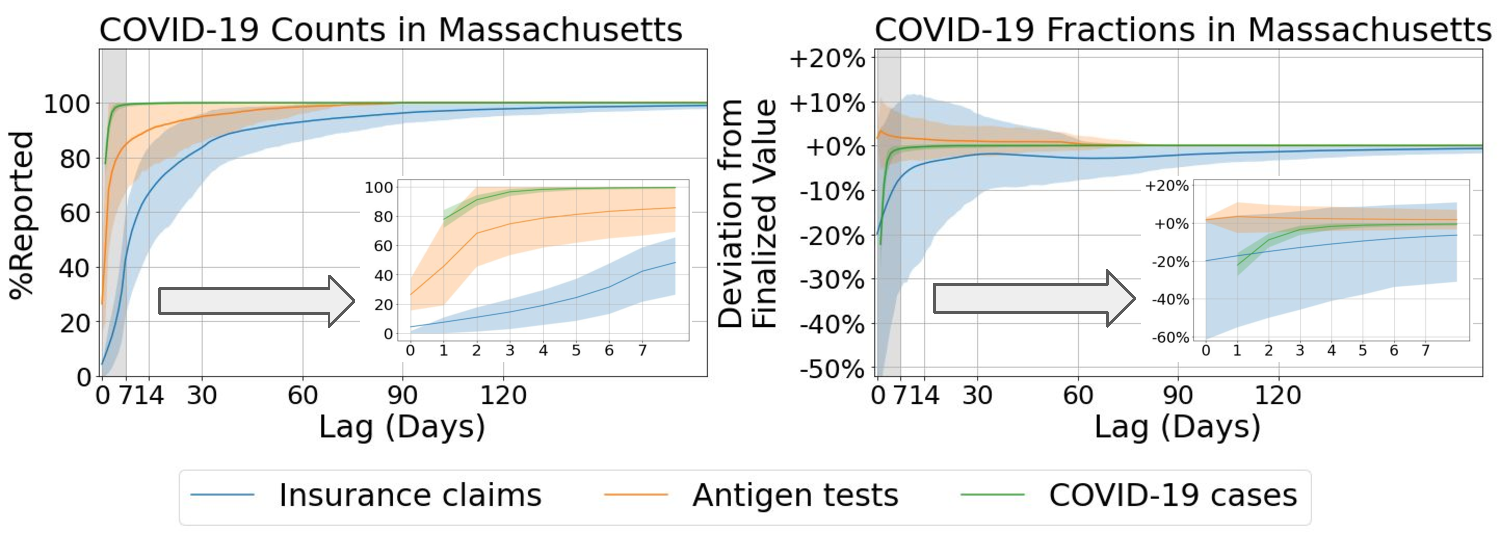
\includegraphics[width=\textwidth]{figs/Intro_fig.pdf}
    \caption{\textit{\textbf{Data revision for different indicators.} Left: Mean percentage of total counts reported, averaged over all reference dates considered, over lags for states in US. The shaded bands correspond to 10\% quantile to 90\% quantile intervals. Right: Mean fraction of COVID-19 fractions normalized by the revised reports 300 days later, averaged over all reference dates considered, over lags for Massachusetts.}}
\end{figure}



